\section{Applying LIME}
\nblink{nhs-chest-xray/analyze/lime.ipynb}
Implementing LIME on the NIH Chest X-ray dataset with the DenseNet model was straightforward. The reference implementation is published on PyPI (Python Packaging Index) and can be installed with the pip Python package manager. Examples how to use LIME with PyTorch are available in the official GitHub repository \cite{limegithub}.


\subsection{Results}
\begin{figure}[H]
\centering
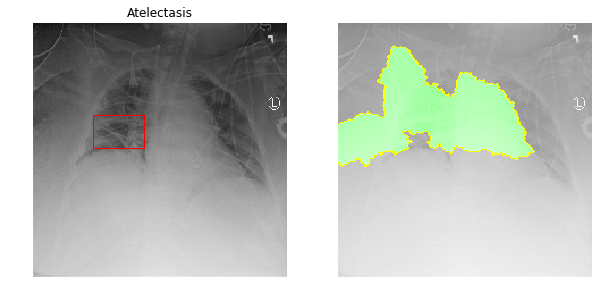
\includegraphics[width=12cm]{chapters/03_classification/images/lime_0.png}
\caption{The left image shows the input image with the bounding box added by a physician. The right image shows LIME superpixels which the network considers important for the classification. The superpixels are at the correct location, but too big in comparison to the bounding box.}
\label{lime_example_1}
\end{figure}

\begin{figure}[H]
\centering
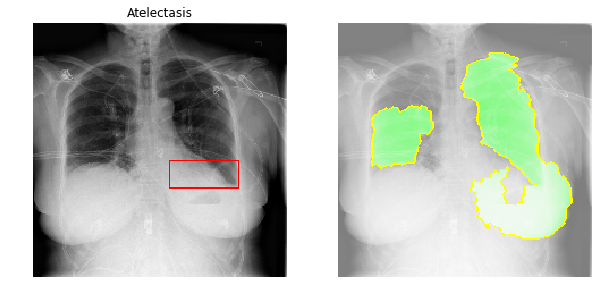
\includegraphics[width=12cm]{chapters/03_classification/images/lime_2.png}
\caption{The left image shows the input image with the bounding box added by a physician. The right image shows LIME superpixels which the network considers important for the classification. Parts of the marked regions are inside the bounding box, but a big part is missing in the center.}
\label{lime_example_2}
\end{figure}

\begin{figure}[H]
\centering
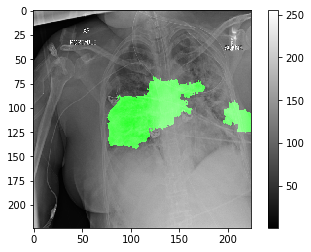
\includegraphics[width=12cm]{chapters/03_classification/images/lime_8.png}
\caption{The left image shows the input image with the bounding box added by a physician. The right image shows LIME superpixels which the network considers important for the classification. The superpixels mostly do not match the bounding box.}
\label{lime_example_3}
\end{figure}

\subsection{LIME configuration}
\nblink{nhs-chest-xray/analyze/lime\_num\_features.ipynb}
LIME has an important configuration parameter, the count of how many superpixels should be returned. Figure \ref{lime_superpixel_count} shows the image from Figure \ref{lime_example_1} with different superpixel counts.

\begin{figure}[H]
\centering
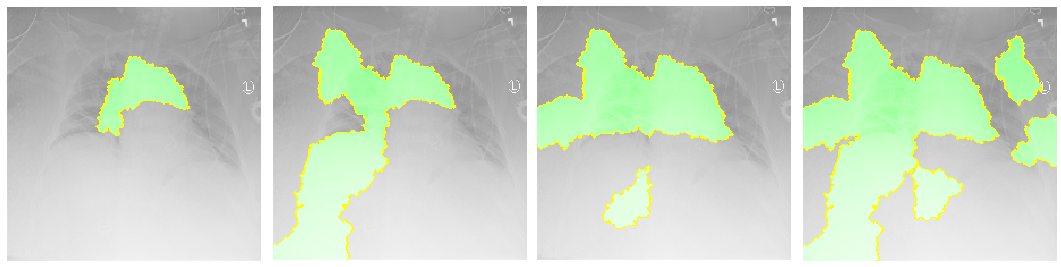
\includegraphics[width=14cm]{chapters/03_classification/images/lime-superpixel.png}
\caption{LIME applied to the first example image from Figure \ref{lime_example_1} with different superpixel counts: 1, 3, 6, 9}
\label{lime_superpixel_count}
\end{figure}

\subsection{Discussion}
The LIME output from Figure \ref{lime_example_1} does match the bounding box, but is much bigger than the bounding box. A smaller superpixel count as seen in Figure \ref{lime_superpixel_count} for the same image reduces the marked region, but is still quite inaccurate. Figure \ref{lime_example_2} and \ref{lime_example_3} show only only parts of the LIME output matching with the bounding box.

\subsection{Conclusion}
The output of the LIME method shows a weak correlation between the bounding boxes provided by physician and the regions the neural network considers important for the output, as shown by LIME superpixels.
